%%%%%%%%%%%%%%%%%%%%%%%%%%%%%%%%%%%%%%%%%%%%%%%%%%%%%%%%%%%%%%%%%%%%%%%%%%%%%%%%
%2345678901234567890123456789012345678901234567890123456789012345678901234567890
%        1         2         3         4         5         6         7         8

\documentclass[letterpaper, 10 pt, conference]{ieeeconf}

\IEEEoverridecommandlockouts
\overrideIEEEmargins

\usepackage[utf8]{inputenc}
\usepackage[T1]{fontenc}
\usepackage{graphicx}
\usepackage{booktabs}
\usepackage{amsmath}
\usepackage{hyperref}
\usepackage{xcolor}
\usepackage{subcaption}
\usepackage{array}
\usepackage{textcomp}
\setlength{\textfloatsep}{6pt plus 1pt minus 2pt}
\setlength{\floatsep}{4pt plus 1pt minus 2pt}
\setlength{\intextsep}{6pt plus 1pt minus 2pt}
\setlength{\abovecaptionskip}{2pt}
\setlength{\belowcaptionskip}{0pt}
\renewcommand{\topfraction}{0.9}
\renewcommand{\bottomfraction}{0.9}
\renewcommand{\textfraction}{0.05}
\renewcommand{\floatpagefraction}{0.85}
\setcounter{topnumber}{4}
\setcounter{bottomnumber}{3}
\setcounter{totalnumber}{8}
\setcounter{dbltopnumber}{3}
\usepackage{placeins}

% Fix for \input in tables with booktabs (LaTeX 2020+ compatibility)
\ExplSyntaxOn
\cs_if_exist:NF \expandableinput
  {
    \cs_new:Npn \expandableinput #1
      { \use:c { @@input } { \file_full_name:n {#1} } }
  }
\AddToHook{env/tabular/begin}
  { \cs_set_eq:NN \input \expandableinput }
\ExplSyntaxOff

\graphicspath{{figures/}}

\title{\LARGE \bf
Unsupervised Learning and Dimensionality Reduction:\\
Clustering, Projection, and Neural Network Analysis\\
on Adult Income and Wine Quality
}

\author{siddartha sagar chinne\\
{\tt\small schinne3@gatech.edu}
}

\begin{document}

\maketitle
\thispagestyle{empty}
\pagestyle{empty}

%%%%%%%%%%%%%%%%%%%%%%%%%%%%%%%%%%%%%%%%%%%%%%%%%%%%%%%%%%%%%%%%%%%%%%%%%%%%%%%%
\begin{abstract}
This report applies K-Means, Expectation Maximization (GMM), and three linear
dimensionality reduction methods --- PCA, ICA, and Random Projection --- to the
Adult Income and Wine Quality datasets studied in prior SL and OL assignments.
The central hypothesis, grounded in prior EDA, is that PCA will improve cluster
quality more on Adult than on Wine: Adult's 104-dimensional one-hot-encoded
space contains structurally collinear redundancy that PCA can compress, while
Wine's 12 compact physicochemical features already exhibit severe quality-class
overlap (silhouette $= -0.074$, prior EDA), leaving little separable structure
for linear projection to expose.  Neural network experiments on Wine confirm
that every DR method degrades Macro-F1 in proportion to compression severity,
while cluster-derived feature augmentation reverses this trend and exceeds the
raw baseline.  t-SNE visualization provides qualitative support for all
quantitative conclusions.
\end{abstract}

%%%%%%%%%%%%%%%%%%%%%%%%%%%%%%%%%%%%%%%%%%%%%%%%%%%%%%%%%%%%%%%%%%%%%%%%%%%%%%%%
\section{Introduction}

This report continues the analysis from the Supervised Learning (SL) and Online
Learning (OL) assignments, reusing the same two datasets and the same
train/validation/test split (60/20/20, \texttt{random\_state=42}).  All
unsupervised models are fit exclusively on the training partition; validation
and test sets remain held out.  Neural network experiments in Steps~4 and~5 use
Wine only, consistent with the assignment requirement to choose a single dataset
for the supervised portion.

\textbf{Hypothesis.}  Prior EDA established two contrasting dataset geometries.
Wine has 12 continuous physicochemical features whose quality-class silhouette
score is $-0.074$, meaning adjacent ratings (e.g., quality 5 vs.\ 6) are more
spatially mixed than a random partition would produce, and both logistic
regression (0.465) and random forest (0.490) fall well below 50\% Macro-F1.
Adult expands to 104 dimensions after one-hot encoding and contains known
collinear feature groups --- \texttt{education} and \texttt{education-num}
encode the same ordinal information redundantly --- while its decision boundary
is nearly linear (only a 1.7\% gap between logistic regression and random
forest)~\cite{kohavi1996}.  From these observations we predict: PCA will
produce a larger relative improvement in cluster quality on Adult than on Wine,
because Adult has genuine redundancy that compression can remove, while Wine's
compact 12-dimensional representation has no such slack.  For the Wine neural
network, compressing already-informative features will likely create an
information bottleneck and degrade Macro-F1.  Whether cluster-derived features
can compensate by encoding coarse structural groupings invisible to linear
methods is an open question entering the experiments.

%%%%%%%%%%%%%%%%%%%%%%%%%%%%%%%%%%%%%%%%%%%%%%%%%%%%%%%%%%%%%%%%%%%%%%%%%%%%%%%%
\section{Exploratory Data Analysis}

\subsection{Adult Income}

The Adult Census dataset~\cite{kohavi1996} contains 45{,}222 samples with 6
numeric and 8 categorical features, expanding to 104 dimensions after one-hot
encoding with a 3:1 class imbalance ($\leq$50K vs.\ $>$50K); we use binary F1
as the primary metric.  A linearity proxy confirms a near-linear decision
boundary: logistic regression achieves 0.809 F1 while random forest reaches
0.826, a gap of only 1.7\%.  Feature--target correlations are weak (maximum
$|r| = 0.24$ for \texttt{age}), and several features are right-skewed.
Structurally redundant OHE groups motivate the hypothesis that PCA will find
many low-variance directions to discard.

\subsection{Wine Quality}

The combined red/white Wine dataset~\cite{cortez2009} contains 6{,}497 samples
with 12 continuous physicochemical features and 8 quality classes (ratings 3--9);
we use Macro-F1 as the primary metric.  Compared to the OL assignment, this
report retains the binary \texttt{type} indicator (red vs.\ white), increasing
the input dimension from 11 to 12; the \texttt{class} duplicate column was
removed as a leakage control.  The silhouette score computed on the 8 quality
labels is $-0.074$ --- adjacent quality classes overlap more than a random
assignment --- and neither LR nor RF exceeds 49\% Macro-F1, confirming a hard
multiclass boundary with no dominant separating direction.

%%%%%%%%%%%%%%%%%%%%%%%%%%%%%%%%%%%%%%%%%%%%%%%%%%%%%%%%%%%%%%%%%%%%%%%%%%%%%%%%
\section{Algorithms and Methodology}

\subsection{Clustering}

K-Means~\cite{lloyd1982} minimizes within-cluster sum of squares via Lloyd's
algorithm using Euclidean distance on standardized features.  We use
$n\_\text{init}=10$ random restarts with k-means++ initialization and sweep
$K \in [2, 20]$, selecting $K$ by the joint behavior of silhouette score,
Calinski-Harabasz (CH), and Davies-Bouldin (DB) without consulting ground-truth
labels.  GMM/EM~\cite{dempster1977} models the data as a mixture of Gaussian
components estimated via the Expectation-Maximization algorithm; it supports
elliptical, overlapping clusters and yields soft posterior probabilities.  We
use diagonal covariance with $\text{reg\_covar}=10^{-3}$ to prevent singularity
in Adult's sparse OHE space, and select component count by minimizing BIC.

\subsection{Dimensionality Reduction}

PCA finds orthogonal directions of maximum variance; we retain the minimum
number of components that cumulatively explain $\geq 90\%$ of variance.
ICA~\cite{hyvarinen2000} seeks statistically independent, non-Gaussian sources
via FastICA with PCA whitening; component count is set to the number of
components whose absolute kurtosis exceeds the median (minimum 2).  Random
Projection~\cite{jl1984} multiplies by a random Gaussian matrix, approximately
preserving pairwise Euclidean distances by the Johnson-Lindenstrauss lemma; we
match RP's target dimension to the PCA selection and sweep 10 random seeds to
characterize stability.

\subsection{Neural Network}

All NN experiments use the same architecture from the OL report: one hidden
layer of 100 ReLU units, cross-entropy loss, Adam optimizer
($\text{lr}=10^{-3}$, $\beta_1=0.9$, $\beta_2=0.999$), batch size 128, 20
epochs, 10 seeds (42--51).  The input dimension varies across variants; all
other hyperparameters are fixed, isolating the effect of the input
transformation.

%%%%%%%%%%%%%%%%%%%%%%%%%%%%%%%%%%%%%%%%%%%%%%%%%%%%%%%%%%%%%%%%%%%%%%%%%%%%%%%%
\section{Step 1: Clustering on Raw Data}

\begin{table}[t]
  \caption{Raw clustering metrics at frozen $K$.
           CH\,$=$\,Calinski-Harabasz\,($\uparrow$);
           DB\,$=$\,Davies-Bouldin\,($\downarrow$); BIC/AIC\,($\downarrow$).}
  \label{tab:phase2}
  \begin{tabular}{llrrrr}
\toprule
Dataset & Algorithm & $K$ & Silhouette & CH / BIC & DB / AIC \\
\midrule
Wine & K-Means & 2 & 0.340 & 1497 & 1.335 \\
Wine & GMM (EM) & 7 & 0.040 & 60841 & 56855 \\
Adult & K-Means & 8 & 0.114 & 2583 & 2.064 \\
Adult & GMM (EM) & 7 & 0.058 & -8290938 & -8610691 \\
\midrule
\multicolumn{6}{l}{\footnotesize CH = Calinski-Harabasz (\textuparrow); DB = Davies-Bouldin (\textdownarrow); BIC/AIC (\textdownarrow)} \\
\bottomrule
\end{tabular}

\end{table}

\begin{figure*}[t]
  \centering
  \begin{subfigure}{0.23\textwidth}
    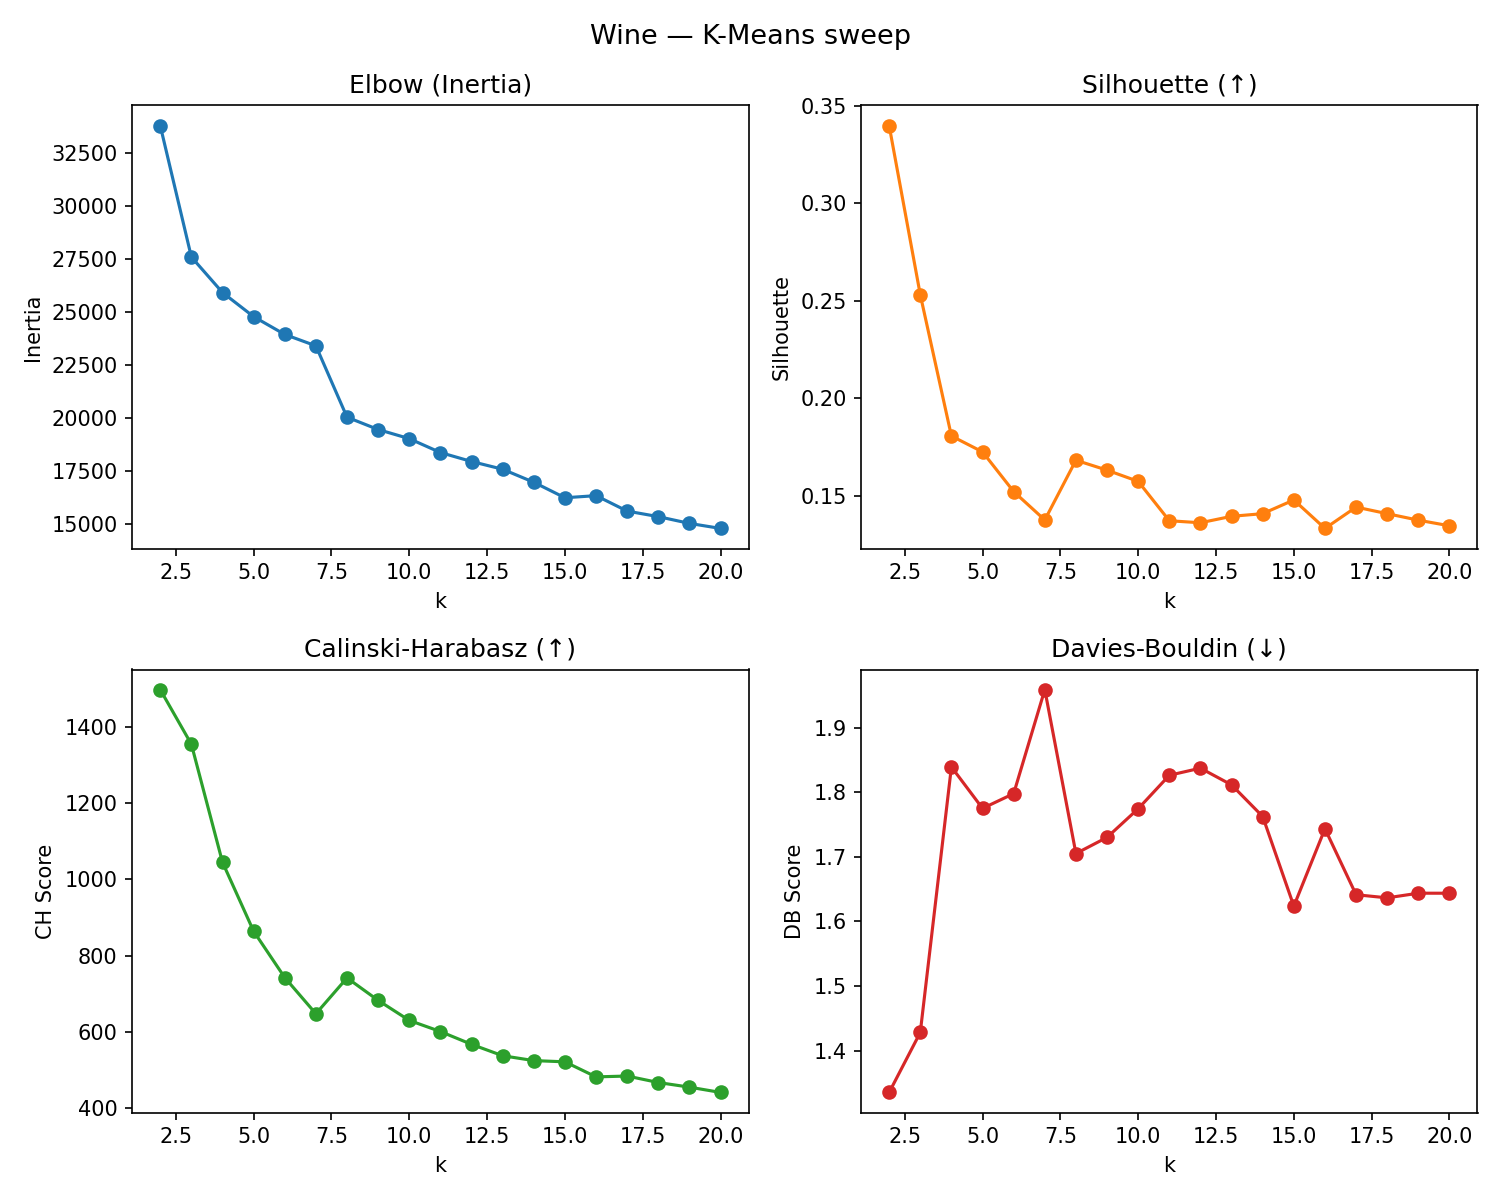
\includegraphics[width=\linewidth]{phase2_clustering/wine_kmeans}
    \caption{Wine K-Means}
  \end{subfigure}
  \hfill
  \begin{subfigure}{0.23\textwidth}
    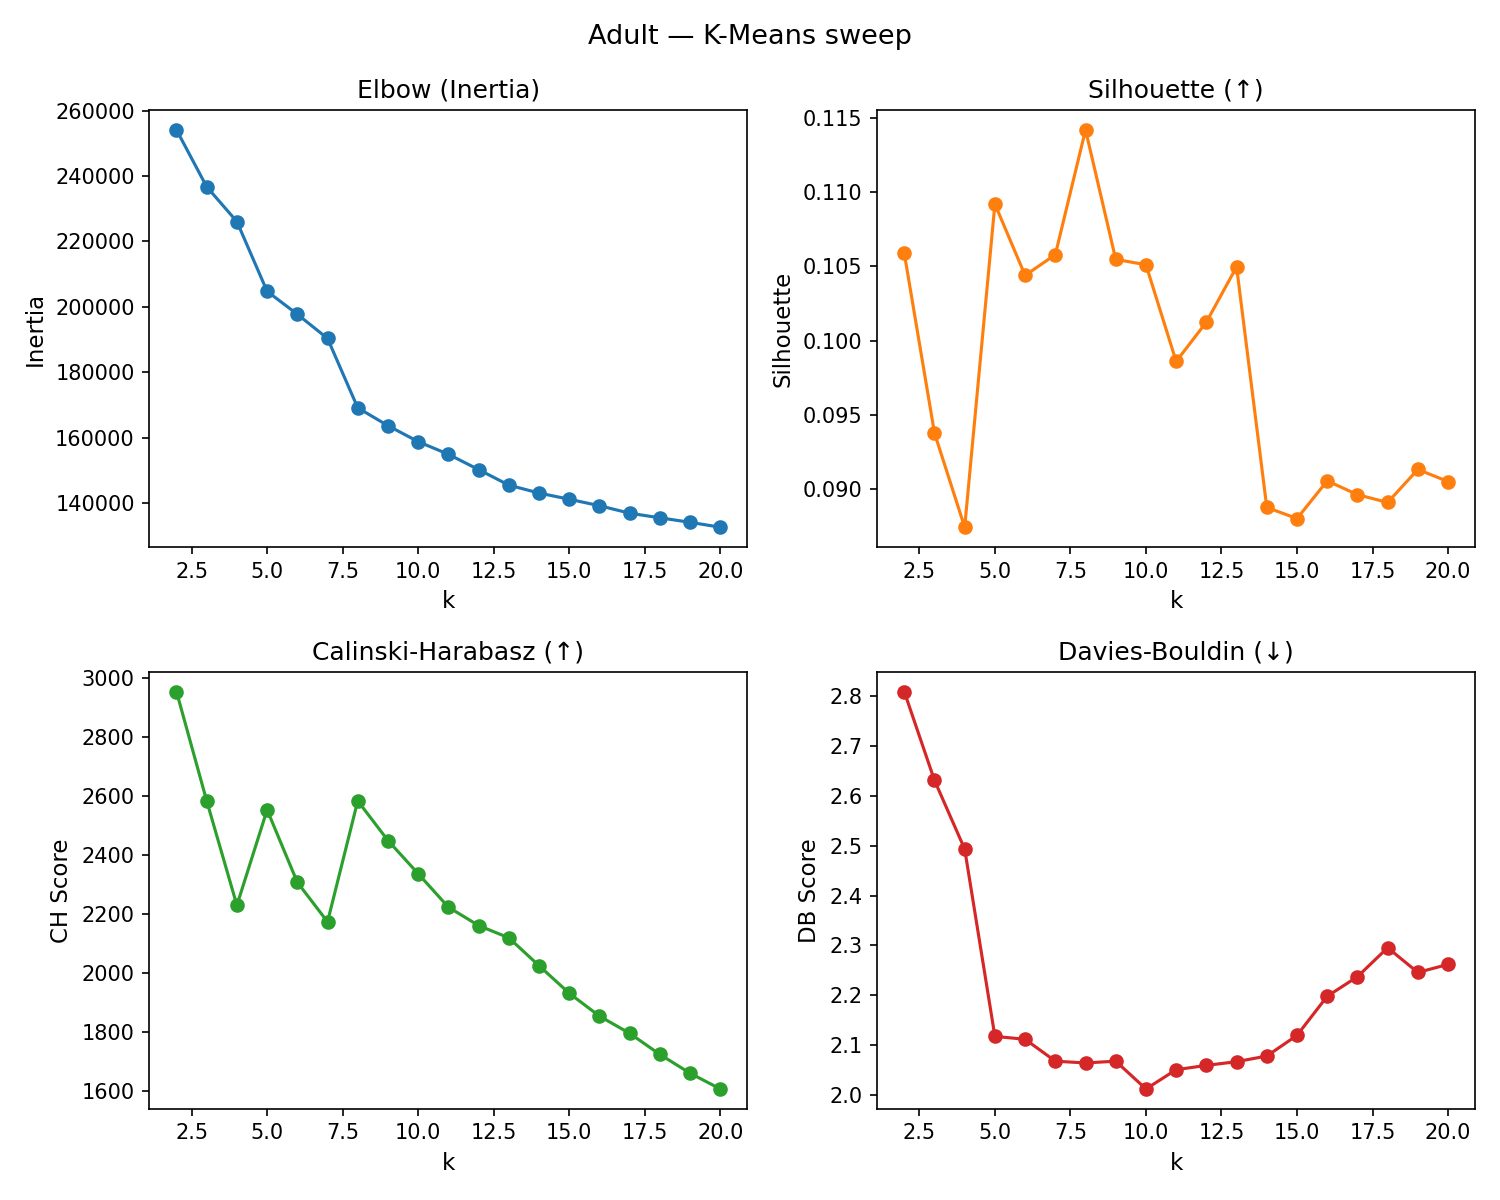
\includegraphics[width=\linewidth]{phase2_clustering/adult_kmeans}
    \caption{Adult K-Means}
  \end{subfigure}
  \hfill
  \begin{subfigure}{0.23\textwidth}
    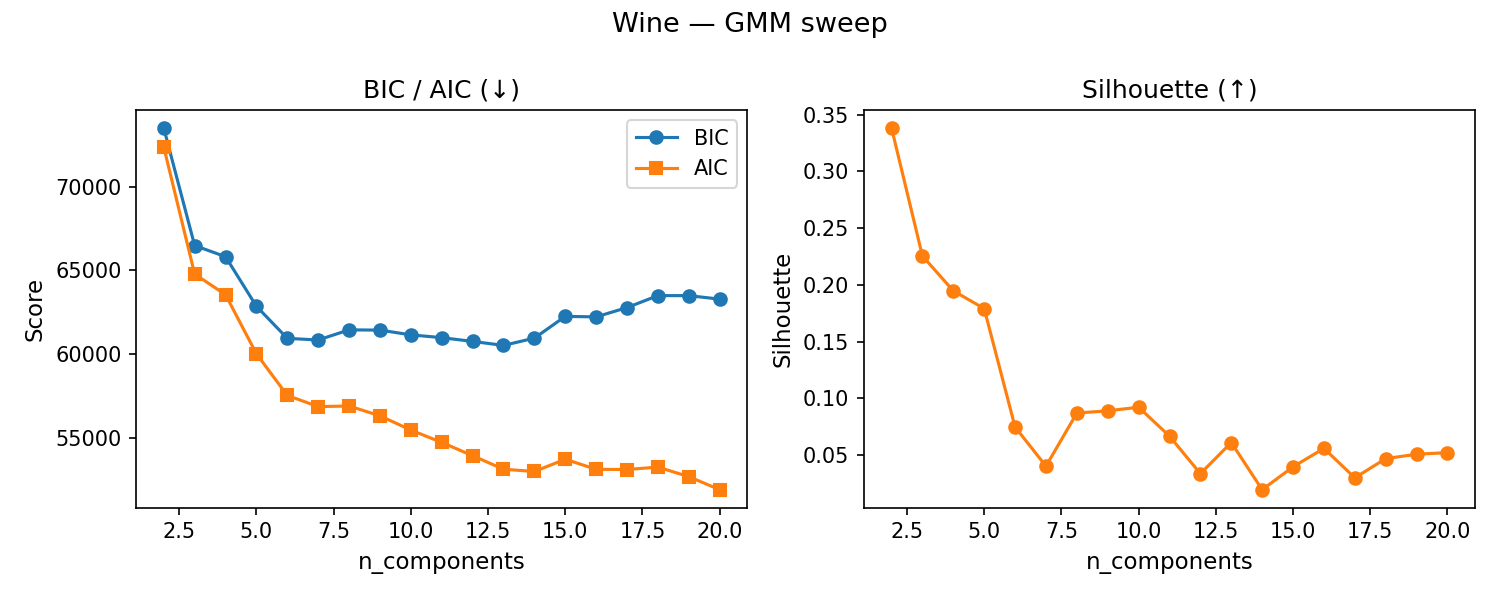
\includegraphics[width=\linewidth]{phase2_clustering/wine_gmm}
    \caption{Wine GMM}
  \end{subfigure}
  \hfill
  \begin{subfigure}{0.23\textwidth}
    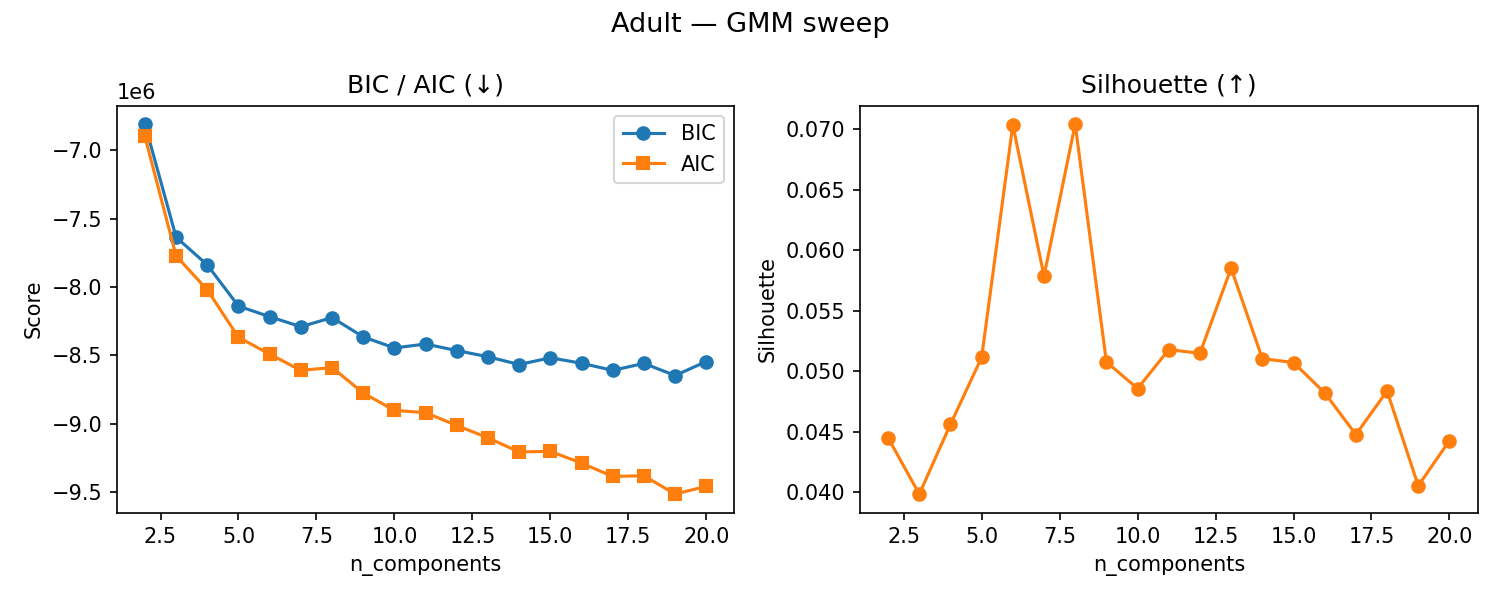
\includegraphics[width=\linewidth]{phase2_clustering/adult_gmm}
    \caption{Adult GMM}
  \end{subfigure}
  \caption{Clustering metric sweeps across $K \in [2,20]$.
  \textbf{Takeaway (K-Means):} Wine peaks sharply at $K\!=\!2$ with silhouette
  declining monotonically --- consistent with one dominant partition (red
  vs.\ white) rather than quality grades.  Adult shows a gradual plateau near
  $K\!=\!8$; the absence of a clean elbow reflects the high-dimensional sparse
  OHE geometry where Euclidean distances are less discriminative.
  \textbf{Takeaway (GMM):} Both datasets select $K\!=\!7$ via BIC minimization.
  Wine's BIC curve is positive and relatively flat, indicating the generative
  model does not fit cleanly at any $K$; Adult's strongly negative BIC confirms
  an excellent generative fit consistent with its near-linear structure.}
  \label{fig:kmeans_sweep}
\end{figure*}

Table~\ref{tab:phase2} and Fig.~\ref{fig:kmeans_sweep} summarize the clustering
results.  Wine K-Means selects $K=2$ at silhouette 0.340 and CH\,=\,1{,}497,
indicating two compact, well-separated macro-clusters.  To determine whether
these clusters align with the ground-truth structure, we computed the Adjusted
Rand Index (ARI) between each cluster assignment and the available labels.
Wine KMeans $K\!=\!2$ achieves ARI\,=\,0.981 against the binary red/white type
label --- near-perfect agreement --- while ARI against the 8 quality classes is
only 0.182.  The clustering has therefore recovered the wine type, not quality,
consistent with the prior EDA finding that quality classes overlap severely.
Wine GMM $K\!=\!7$ achieves ARI\,=\,0.118 against quality and ARI\,=\,0.218
against type, indicating its seven components span both wine types without
cleanly recovering either structure; EM finds a statistically optimal generative
decomposition, but the resulting components do not correspond to compact or
label-aligned spatial regions.

Adult K-Means selects $K=8$ at silhouette 0.114 --- low, but consistent with
high-dimensional sparse geometry where Euclidean distances are less
discriminative.  Adult KMeans $K\!=\!8$ achieves ARI\,=\,0.059 against the
binary income label, and Adult GMM $K\!=\!7$ achieves ARI\,=\,0.079 ---  both
near zero, confirming that the cluster structure reflects feature co-occurrence
patterns in the OHE space rather than the supervised income boundary.  Adult GMM
achieves a strongly negative BIC ($-8.29\!\times\!10^6$) at $K=7$, indicating
an excellent generative fit; the negative sign is expected for large-$n$
datasets where the log-likelihood term dominates the BIC penalty.  The contrast
between Adult's excellent BIC and its near-zero ARI illustrates that generative
fit and label-aligned cluster quality are independent objectives.

%%%%%%%%%%%%%%%%%%%%%%%%%%%%%%%%%%%%%%%%%%%%%%%%%%%%%%%%%%%%%%%%%%%%%%%%%%%%%%%%
\section{Step 2: Dimensionality Reduction}

\begin{table}[t]
  \caption{Frozen component counts per dataset and DR method.}
  \label{tab:phase3}
  \begin{tabular}{llrl}
\toprule
Dataset & Method & $d$ & Selection criterion \\
\midrule
Wine & PCA & 8 & Cumulative variance $\geq 90\%$ \\
Wine & ICA & 4 & Above-median $|$kurtosis$|$ (floor 2) \\
Wine & RP & 8 & = PCA target dim \\
Adult & PCA & 22 & Cumulative variance $\geq 90\%$ \\
Adult & ICA & 11 & Above-median $|$kurtosis$|$ (floor 2) \\
Adult & RP & 22 & = PCA target dim \\
\bottomrule
\end{tabular}

\end{table}

\begin{figure}[t]
  \centering
  \begin{subfigure}{0.48\linewidth}
    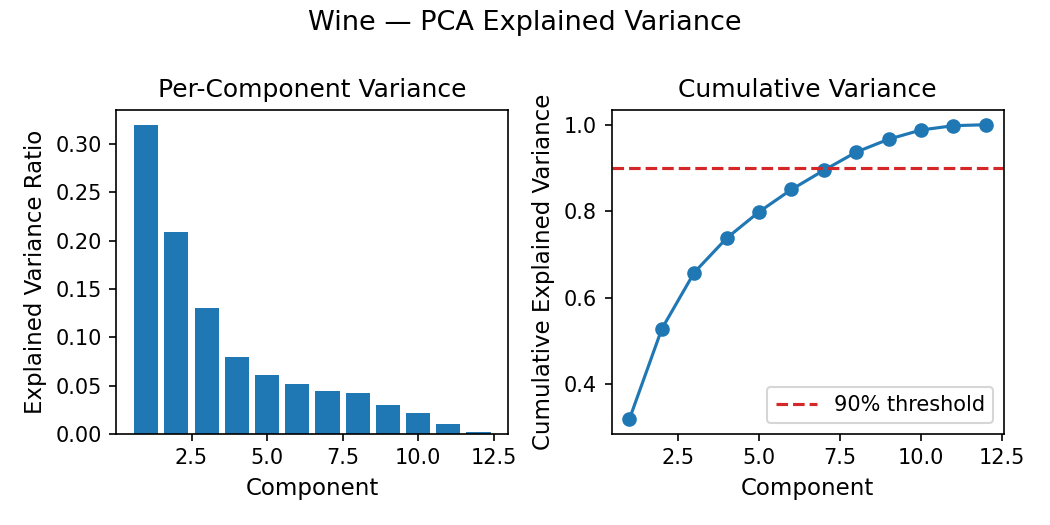
\includegraphics[width=\linewidth]{phase3_reduction/wine_pca_variance}
    \caption{Wine PCA}
  \end{subfigure}
  \hfill
  \begin{subfigure}{0.48\linewidth}
    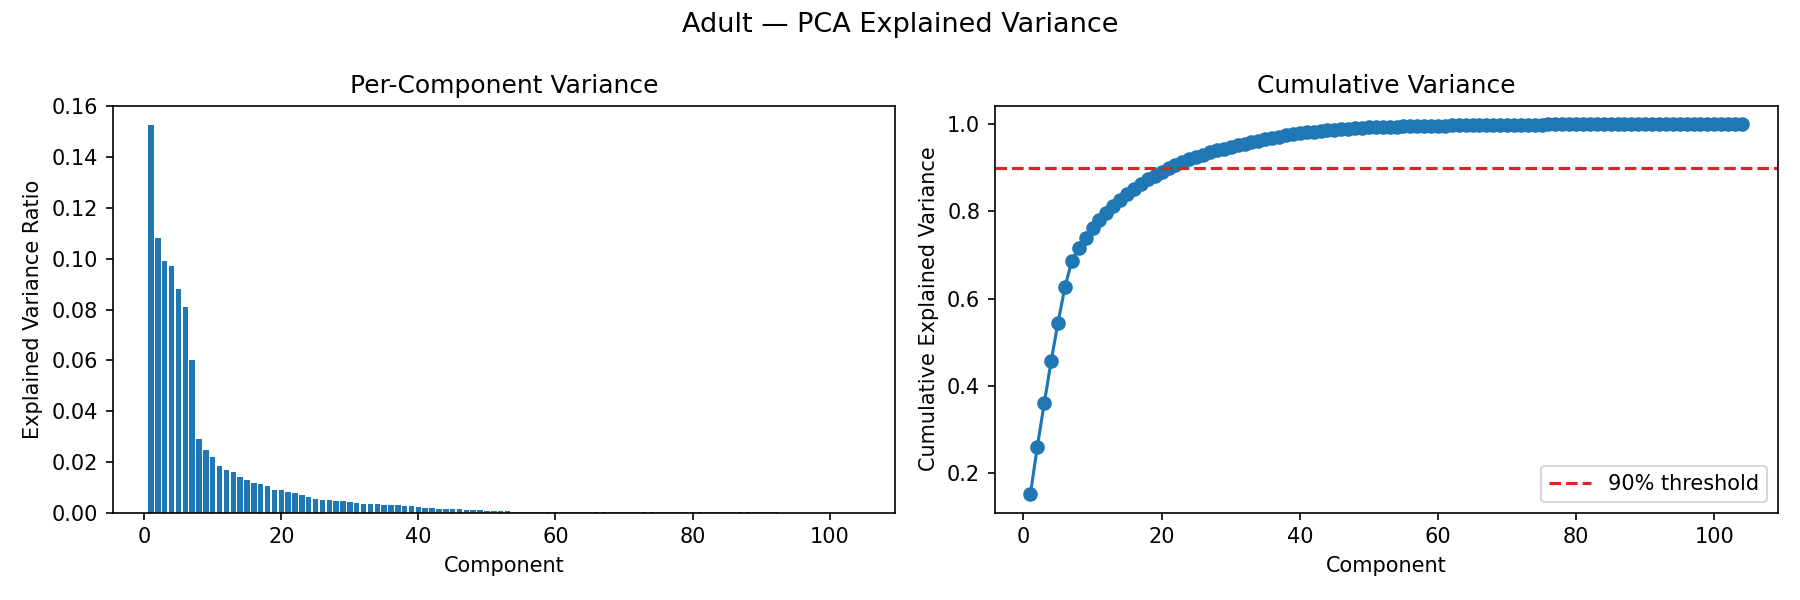
\includegraphics[width=\linewidth]{phase3_reduction/adult_pca_variance}
    \caption{Adult PCA}
  \end{subfigure}
  \caption{Cumulative explained variance vs.\ component count.
  \textbf{Takeaway:} Wine reaches 90\% at $d\!=\!8$ of 12 features
  (PC1\,=\,31.9\%), retaining 67\% of dimensions.  Adult requires $d\!=\!22$
  of 104 features with a notably flat spectrum (PC1\,=\,15.3\%), compressing to
  21\% of dimensions --- confirming that Adult's OHE redundancy is distributed
  across many correlated axes rather than concentrated in a few dominant ones.}
  \label{fig:pca}
\end{figure}

\begin{figure}[t]
  \centering
  \begin{subfigure}{0.48\linewidth}
    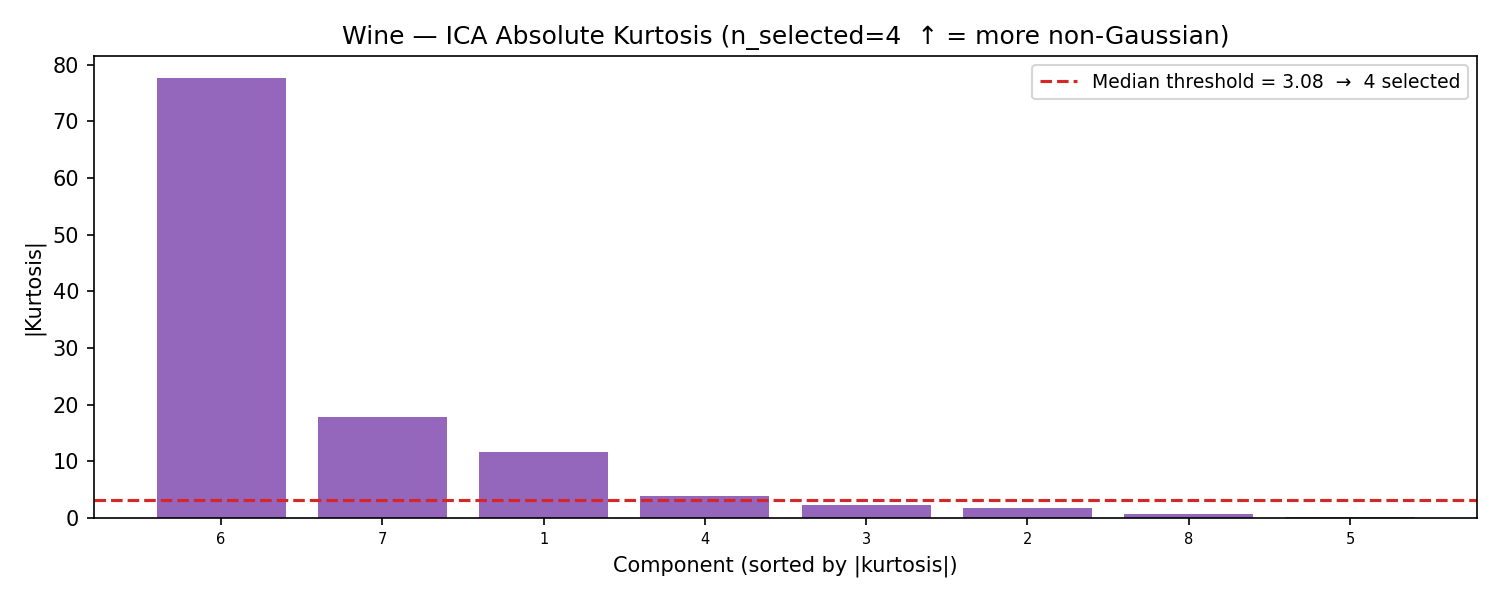
\includegraphics[width=\linewidth]{phase3_reduction/wine_ica_kurtosis}
    \caption{Wine ICA ($n_{\text{sel}}\!=\!4$)}
  \end{subfigure}
  \hfill
  \begin{subfigure}{0.48\linewidth}
    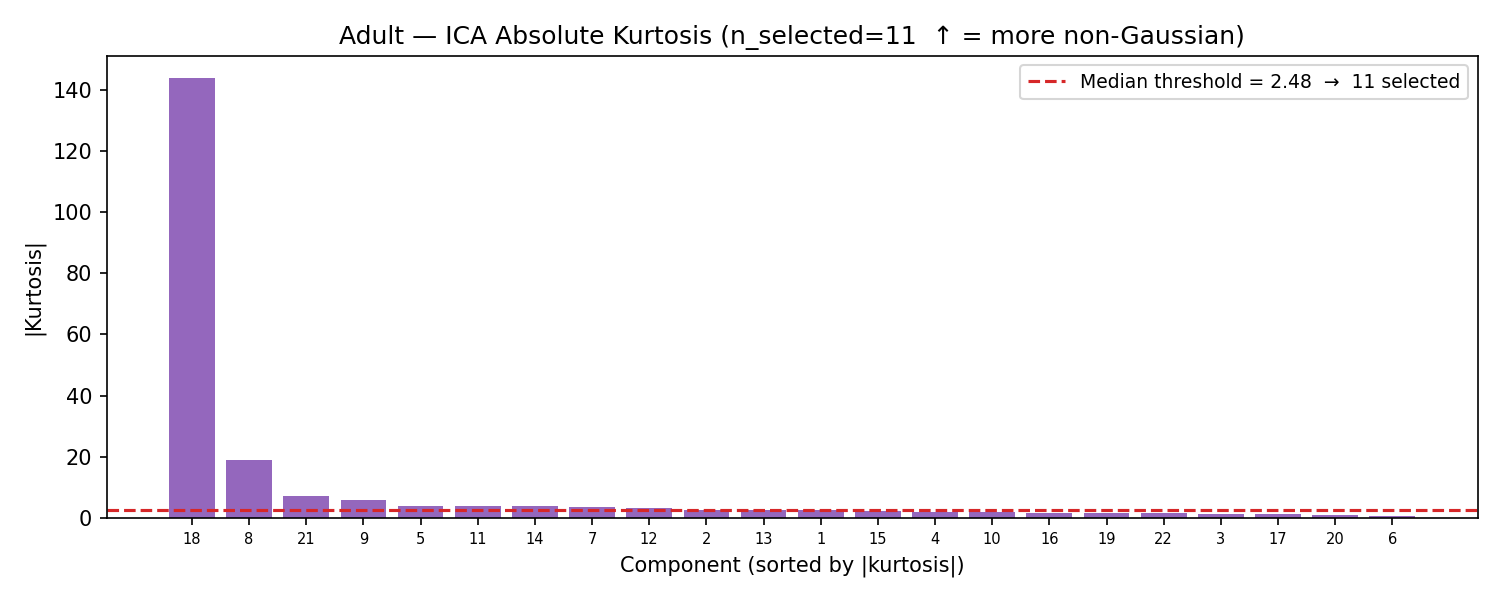
\includegraphics[width=\linewidth]{phase3_reduction/adult_ica_kurtosis}
    \caption{Adult ICA ($n_{\text{sel}}\!=\!11$)}
  \end{subfigure}
  \caption{Absolute kurtosis per ICA component (sorted descending).  Dashed line
  marks the median threshold; components above it are retained.
  \textbf{Takeaway:} Wine retains only 4 components --- most are near-Gaussian
  (low kurtosis), suggesting that Wine's quality signal is not encoded in highly
  non-Gaussian independent sources.  Adult retains 11, reflecting richer
  non-Gaussian structure in its mixed categorical-numeric space.}
  \label{fig:ica}
\end{figure}

\begin{figure}[t]
  \centering
  \begin{subfigure}{0.48\linewidth}
    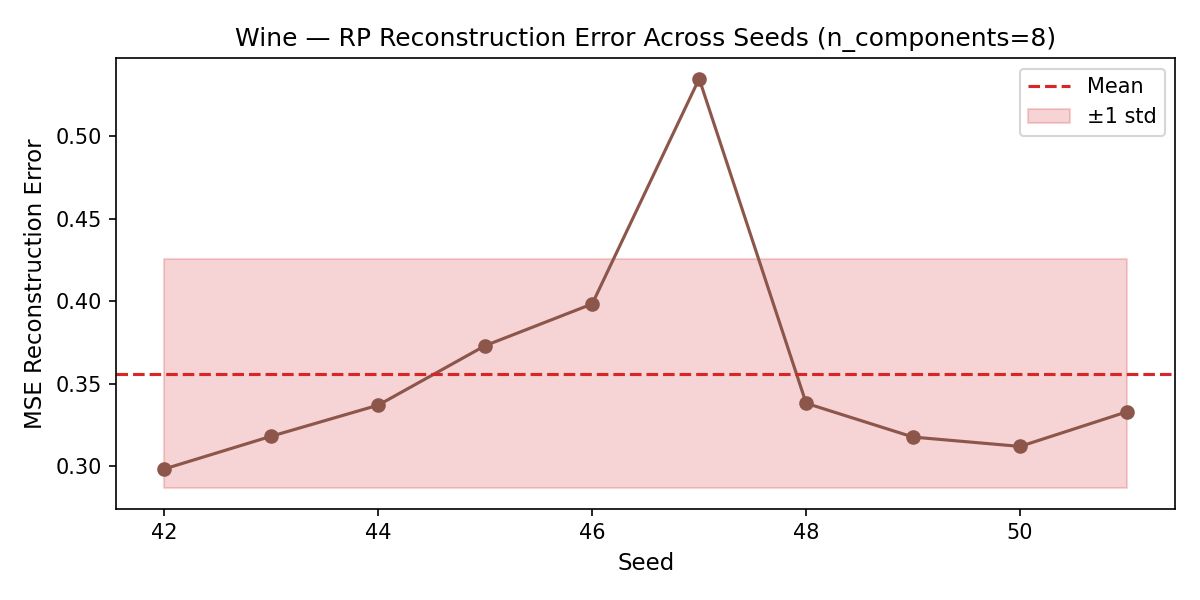
\includegraphics[width=\linewidth]{phase3_reduction/wine_rp_stability}
    \caption{Wine RP ($d\!=\!8$)}
  \end{subfigure}
  \hfill
  \begin{subfigure}{0.48\linewidth}
    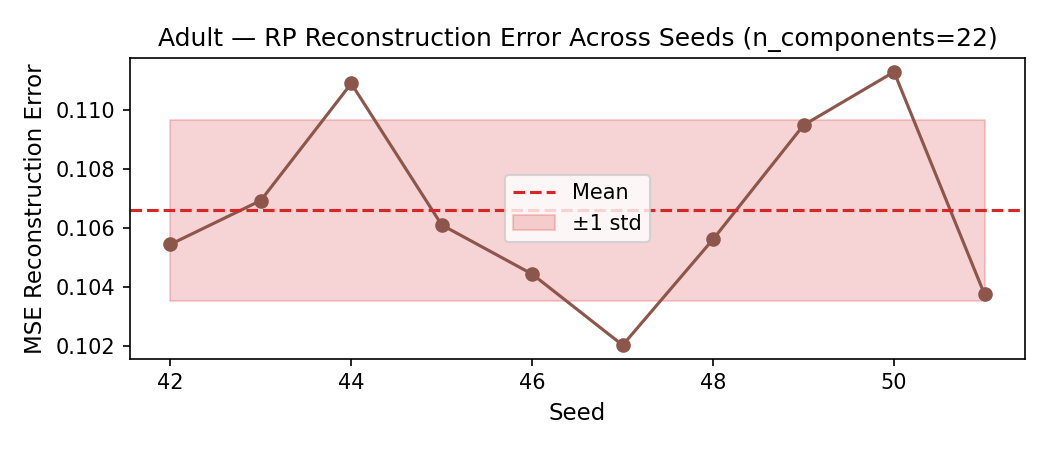
\includegraphics[width=\linewidth]{phase3_reduction/adult_rp_stability}
    \caption{Adult RP ($d\!=\!22$)}
  \end{subfigure}
  \caption{RP reconstruction error vs.\ component count across 10 random seeds
  (shaded band $=\pm1$ SD).  \textbf{Takeaway:} Both datasets are stable at
  the selected target dimension.  Adult's error is more sensitive to small $d$
  due to higher ambient dimensionality: projecting 104 binary-sparse dimensions
  to fewer than 10 loses substantial pairwise distance information, while Wine
  at 12 dense continuous dimensions is more forgiving of aggressive projection.}
  \label{fig:rp}
\end{figure}

Table~\ref{tab:phase3} and Figs.~\ref{fig:pca}--\ref{fig:rp} summarize the DR
analysis.  The PCA eigenvalue spectra in Fig.~\ref{fig:pca} expose the
compression-ratio disparity at the heart of the hypothesis.  Wine retains 8 of
12 principal components (67\%), a modest compression in a space that was already
compact; PC1 capturing 31.9\% indicates moderate collinearity, consistent with
the known correlations among acidity, pH, and density in physicochemical data.
Adult requires 22 of 104 components (21\%), a $4.7\!\times$ reduction; its flat
spectrum (PC1\,=\,15.3\%) reflects OHE redundancy distributed across the entire
feature matrix rather than concentrated in a dominant direction.  The intrinsic
dimensionality of Adult's training data is therefore far lower than its nominal
104 dimensions, which explains why PCA compression benefits downstream tasks
more on Adult than on Wine.

\textbf{Component loadings.}  Figs.~\ref{fig:wine_loadings} and~\ref{fig:adult_loadings}
show the feature loadings of the top PCA components and retained ICA sources.
For Wine, PC1 loads most heavily on \texttt{type} (red/white indicator),
\texttt{total SO\textsubscript{2}}, and \texttt{volatile acidity}: the first
principal direction is essentially the red-vs-white split, which directly
explains why Wine KMeans $K\!=\!2$ under PCA reproduces the raw partition with
ARI\,=\,0.998.  PC2 captures the density--alcohol--residual sugar triangle, a
known physicochemical constraint in wine (higher alcohol density corresponds to
lower residual sugar).  PC3 separates the acidity cluster (citric acid, pH,
fixed acidity), reflecting a third independent axis of wine chemistry.  For
Adult, PC1 and PC2 both load heavily on \texttt{education-num}, \texttt{age},
and \texttt{relationship\_Husband} --- the socioeconomic axis most correlated
with income --- while PC3 surfaces \texttt{capital-gain} and
\texttt{capital-loss} as an independent financial axis.  The Wine ICA sources
(Fig.~\ref{fig:wine_loadings}, right) recover interpretable directions:
IC2 mirrors the density--alcohol--sugar axis found in PC2, and IC3 mixes
\texttt{volatile acidity}, \texttt{citric acid}, and \texttt{type}, suggesting
that ICA separates the acidity-type confound that PCA compresses into PC1.

\begin{figure}[t]
  \centering
  \begin{subfigure}{0.48\linewidth}
    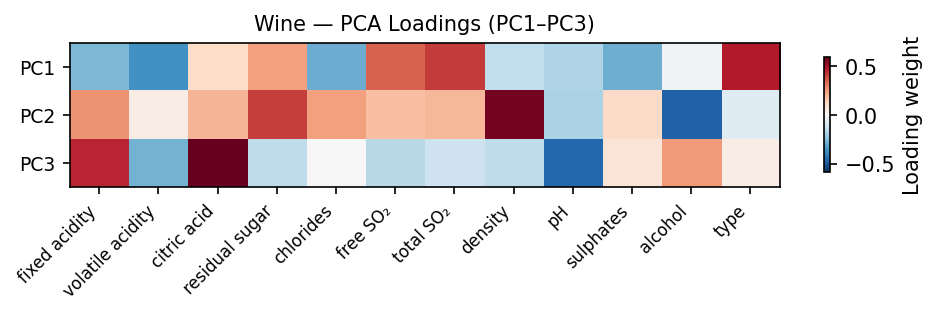
\includegraphics[width=\linewidth]{analysis/wine_pca_loadings}
    \caption{Wine PCA (PC1--3)}
  \end{subfigure}
  \hfill
  \begin{subfigure}{0.48\linewidth}
    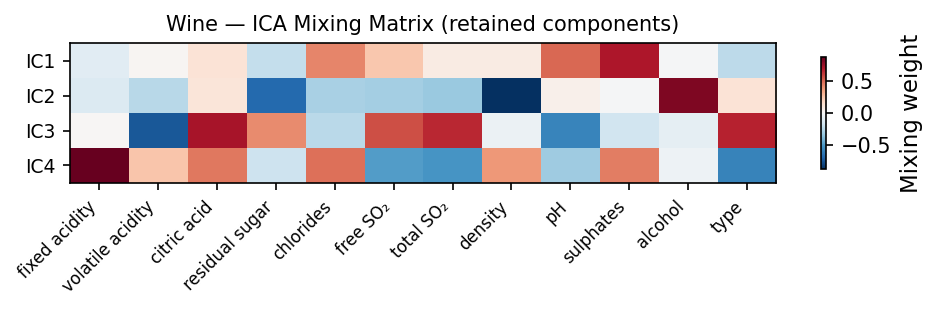
\includegraphics[width=\linewidth]{analysis/wine_ica_loadings}
    \caption{Wine ICA (IC1--4)}
  \end{subfigure}
  \caption{Wine PCA component loadings and ICA mixing matrix.  Red\,=\,negative
  weight, blue\,=\,positive.  \textbf{Takeaway:} PC1 is dominated by
  \texttt{type} (red/white) and SO\textsubscript{2} — the direction that
  K-Means exploits to recover the red/white split.  ICA IC2 independently
  recovers the density--alcohol--sugar axis, demonstrating that ICA finds
  chemically meaningful independent sources distinct from PCA's variance-ordered
  projections.}
  \label{fig:wine_loadings}
\end{figure}

\begin{figure}[t]
  \centering
  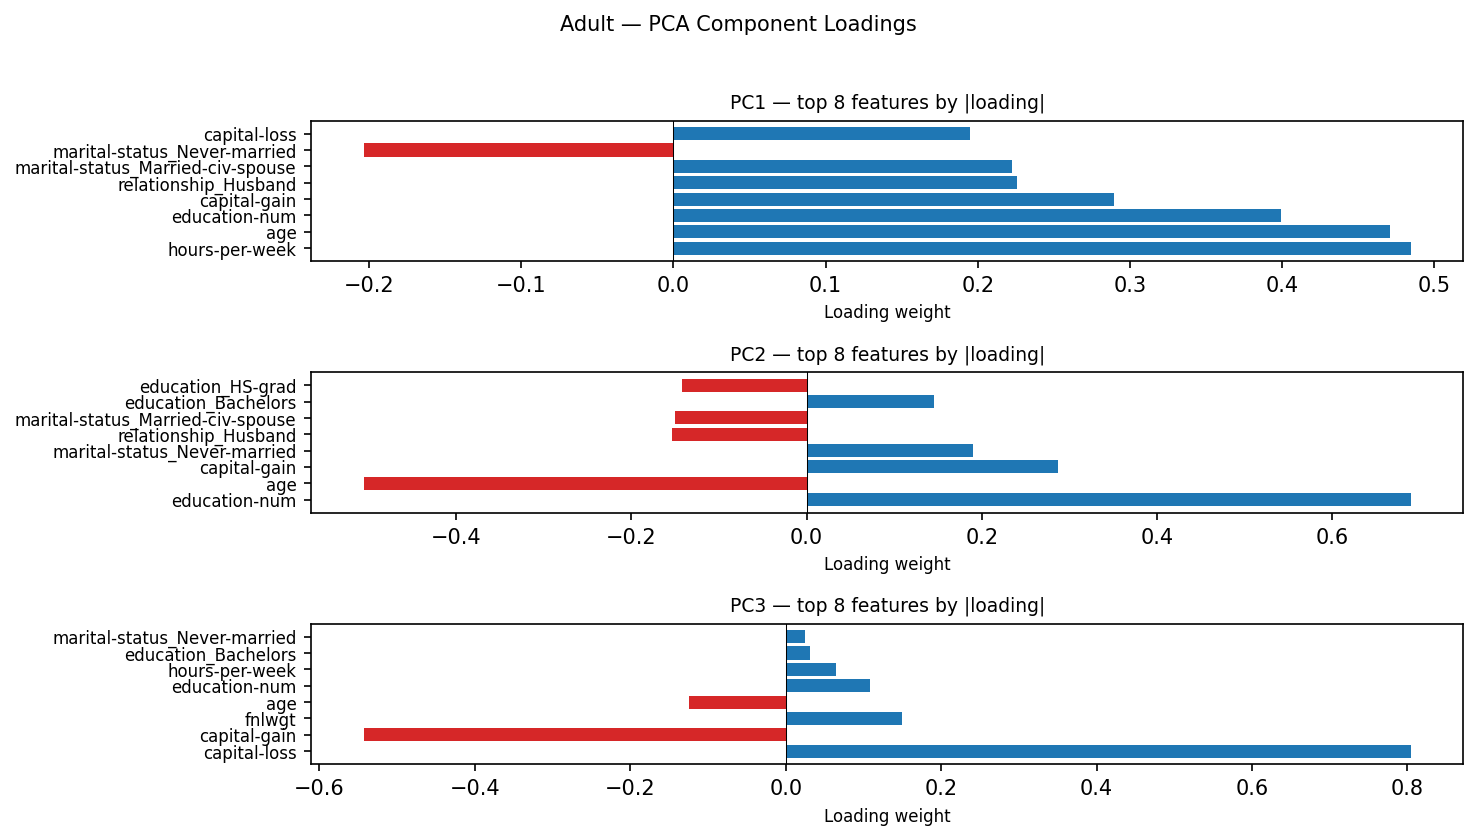
\includegraphics[width=\linewidth]{analysis/adult_pca_loadings}
  \caption{Adult PCA: top-8 features by absolute loading for PC1--3.
  \textbf{Takeaway:} PC1--2 both load on \texttt{education-num},
  \texttt{age}, and \texttt{relationship\_Husband} --- the socioeconomic axis
  most correlated with income --- confirming that PCA compresses the redundant
  OHE education encoding (\texttt{education} vs.\ \texttt{education-num}) into
  a single dominant direction.  PC3 surfaces an independent capital-gains axis.}
  \label{fig:adult_loadings}
\end{figure}

ICA (Fig.~\ref{fig:ica}) corroborates this picture from an independence
perspective.  The above-median kurtosis threshold is grounded in
Hyv\"{a}rinen and Oja's criterion that FastICA sources are meaningful when
they maximize non-Gaussianity~\cite{hyvarinen2000}; the median separates the
near-Gaussian tail from the genuinely non-Gaussian sources the algorithm
recovers.  Wine retains only 4 of 12 components above this threshold, meaning
most features behave nearly Gaussian after whitening --- no strong independent
non-Gaussian sources exist.  Adult retains 11 of 22 whitened components,
reflecting the richer mixture of right-skewed numeric features and binary OHE
indicators whose distributions are far from Gaussian.

Random Projection (Fig.~\ref{fig:rp}) is stable across seeds at the target
dimensions for both datasets, validating the Johnson-Lindenstrauss guarantee.
Adult's steeper reconstruction-error curve at small $d$ confirms that its
ambient space has higher effective dimensionality: random projections to fewer
than $\sim$15 dimensions discard a substantial fraction of pairwise distance
information, whereas Wine's errors remain low even at aggressive compression.
The stability bands in both plots confirm that the specific random matrix
realization does not materially affect the preserved geometry at the selected
target dimensions.  Target dimension for RP is deliberately matched to the PCA
selection ($d\!=\!8$ for Wine, $d\!=\!22$ for Adult) to hold $d$ constant
across methods, enabling a fair downstream comparison in Steps~3 and~4; RP's
Johnson-Lindenstrauss bound could in principle suggest a different optimal $d$,
but fixing it to PCA's isolates the effect of projection type rather than
dimensionality.

%%%%%%%%%%%%%%%%%%%%%%%%%%%%%%%%%%%%%%%%%%%%%%%%%%%%%%%%%%%%%%%%%%%%%%%%%%%%%%%%
\section{Step 3: Clustering in Reduced Spaces}

\begin{table}[t]
  \caption{Silhouette in reduced spaces vs.\ raw baseline.  Bold\,=\,best per
           row.}
  \label{tab:phase4}
  \begin{tabular}{lrrrr}
\toprule
Dataset \& Clusterer & Raw & PCA & ICA & RP \\
\midrule
Wine KMeans & 0.340 & \textbf{0.356} & 0.194 & 0.260 \\
Wine GMM & 0.040 & 0.112 & \textbf{0.225} & 0.099 \\
Adult KMeans & 0.114 & \textbf{0.140} & 0.137 & 0.139 \\
Adult GMM & 0.058 & 0.105 & \textbf{0.121} & 0.039 \\
\multicolumn{5}{l}{\footnotesize Bold = best silhouette per row.} \\
\bottomrule
\end{tabular}

\end{table}

\begin{figure*}[t]
  \centering
  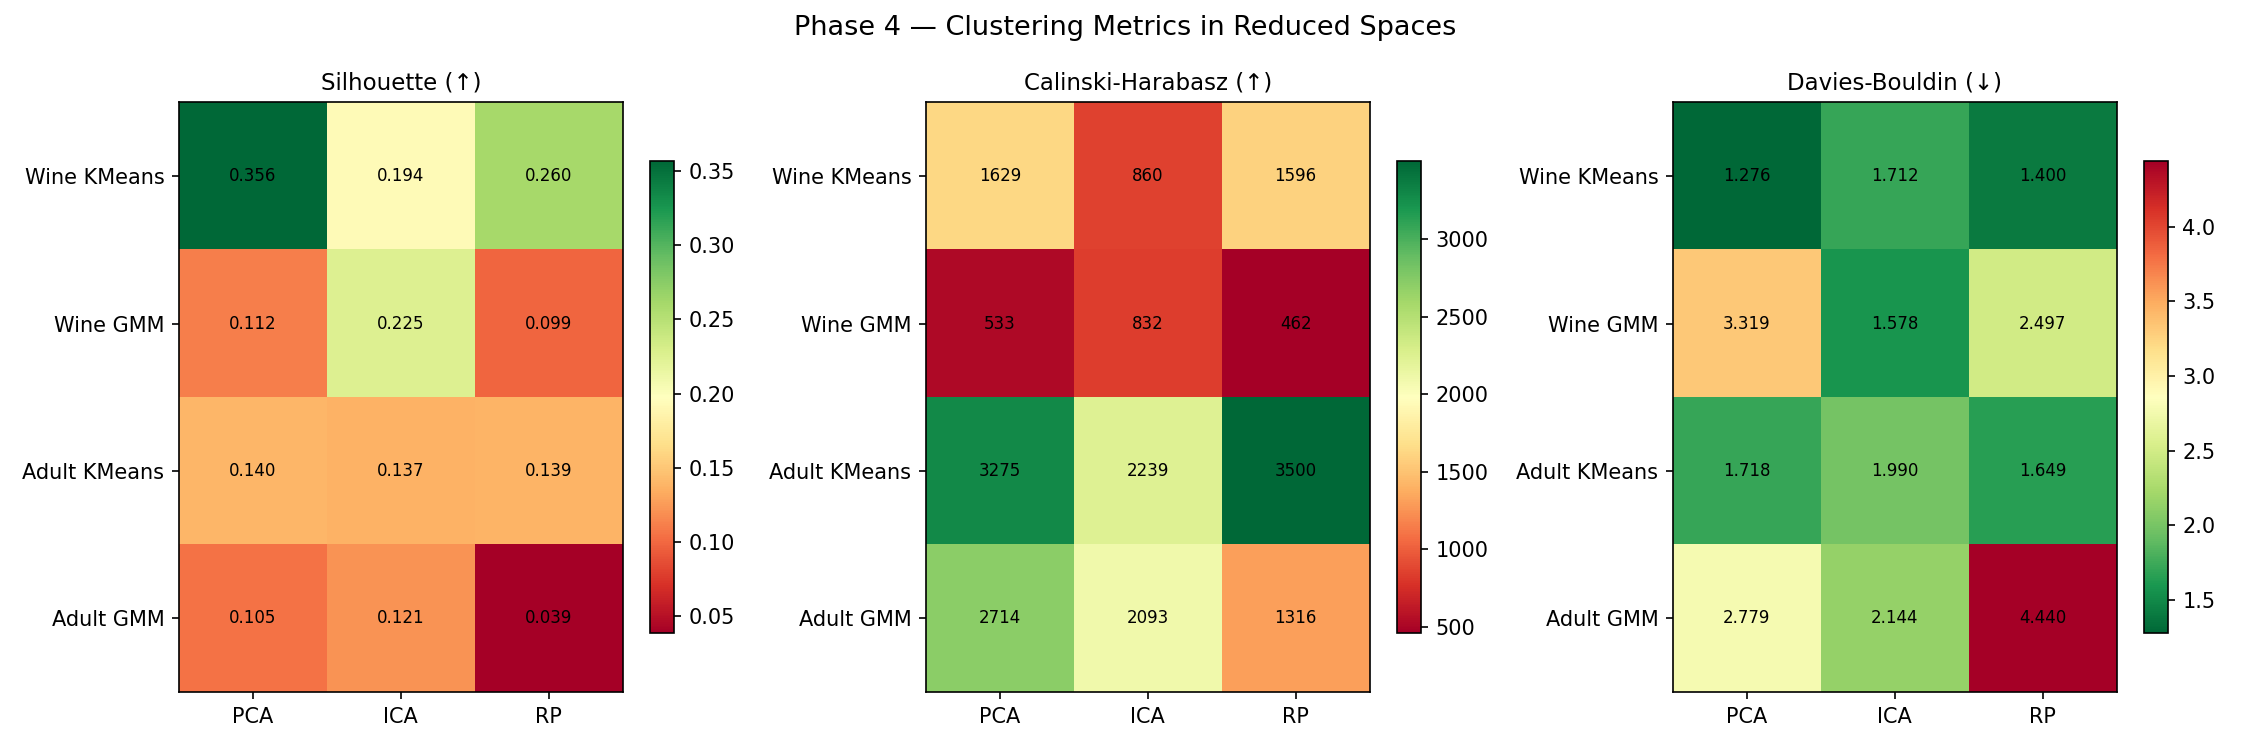
\includegraphics[width=0.88\textwidth]{phase4_clustering/phase4_clustering_heatmap}
  \caption{Per-metric clustering quality across all 12 DR-clusterer combinations
  (each column uses its own color scale).  \textbf{Takeaway:} PCA consistently
  strengthens K-Means silhouette on both datasets while ICA produces the most
  pronounced GMM improvement.  RP tracks PCA closely for Adult K-Means but
  falls short on Wine, where random projections of a compact 12-d space
  introduce more noise than PCA's optimized axes.}
  \label{fig:heatmap}
\end{figure*}

Table~\ref{tab:phase4} and Fig.~\ref{fig:heatmap} present the silhouette
comparison.  The hypothesis is directionally confirmed: Adult K-Means gains
$+23\%$ silhouette under PCA ($0.114 \to 0.140$) while Wine K-Means gains only
$+4.7\%$ ($0.340 \to 0.356$).  The gap is explained by compression ratios:
PCA removes 79\% of Adult's dimensions but only 33\% of Wine's, and the
additional denoising in Adult's space allows K-Means' Euclidean metric to find
tighter, more separated clusters.

The largest single result in the table is Wine GMM under ICA: silhouette
improves from 0.040 to 0.225, a $+463\%$ gain that PCA achieves only partially
(0.112, $+176\%$).  This divergence reflects algorithm geometry.  ICA
maximizes statistical independence via non-Gaussianity, producing a latent space
where mixture components are more separated than in the PCA subspace.  GMM's
Gaussian mixture formulation is naturally aligned with this structure, while
K-Means' spherical Voronoi assumption cannot exploit the non-Gaussian geometry.
The same pairing advantage appears on Adult: ICA gives GMM a $+109\%$ gain
(0.058 to 0.121) compared to PCA's $+81\%$ (0.105), though both methods
substantially improve Adult GMM.

RP matches PCA for Adult K-Means (silhouette 0.139 vs.\ 0.140), consistent with
the Johnson-Lindenstrauss guarantee that pairwise Euclidean distances are
approximately preserved.  On Wine, RP (0.260) falls below PCA (0.356) for
K-Means: projecting an already-compact 12-d space with a random matrix
introduces variance-unweighted noise that PCA's sorted eigendecomposition
avoids.  ICA ($d\!=\!4$) produces the worst Wine K-Means result (0.194),
because four components are insufficient to represent the two-cluster spatial
separation that requires $\sim$8 dimensions.

The Calinski-Harabasz and Davies-Bouldin metrics in Fig.~\ref{fig:heatmap} tell
a consistent story with silhouette: wherever silhouette improves under a given
DR method, CH increases and DB decreases in the same cell, confirming that the
quality gains are not artifacts of any single metric's geometric assumptions.
The one notable divergence is Adult GMM under RP, where silhouette (0.039) is
the lowest of all Adult GMM combinations yet DB remains moderate --- reflecting
that RP's random projection introduces cluster boundary noise that silhouette
penalizes heavily but DB, averaging over within-cluster dispersion, is less
sensitive to.

\textbf{Cluster membership stability.}  To determine whether DR produces the
same clusters as raw-space clustering or fundamentally different ones, we
computed ARI between raw and reduced cluster assignments for each combination.
Wine KMeans under PCA achieves ARI\,=\,0.998 --- the $K\!=\!2$ red/white
partition is essentially identical before and after PCA compression, because
the dominant variance direction that PCA PC1 captures (31.9\%) is exactly the
direction that separates the two macro-clusters.  The silhouette improvement
($+4.7\%$) therefore reflects a cleaner version of the same partition rather
than a different grouping.  Wine KMeans under ICA, by contrast, achieves
ARI\,=\,$-0.010$ --- the assignment is entirely different, which directly
explains the silhouette drop (0.340 to 0.194): four ICA components cannot
represent the two-cluster spatial separation that requires $\sim$8 dimensions.
Adult KMeans under PCA achieves ARI\,=\,0.804, confirming that PCA's
denoising preserves most of the raw partition while tightening cluster
boundaries enough to improve silhouette by 23\%.  GMM combinations across all
DR methods show moderate ARI values (0.24--0.50), reflecting that EM's soft
assignments are sensitive to the geometry of the projected space and naturally
reorganize around the new covariance structure --- which is why ICA can
dramatically improve GMM silhouette even while producing cluster memberships
that differ substantially from the raw solution.

%%%%%%%%%%%%%%%%%%%%%%%%%%%%%%%%%%%%%%%%%%%%%%%%%%%%%%%%%%%%%%%%%%%%%%%%%%%%%%%%
\section{Steps 4 \& 5: Neural Network Experiments on Wine}

\begin{table}[t]
  \caption{NN Macro-F1 on DR-reduced Wine inputs (10 seeds, 42--51).}
  \label{tab:phase5}
  \begin{tabular}{lrrrrl}
\toprule
Variant & $d_{\mathrm{in}}$ & Mean F1 & Std & Min & Max \\
\midrule
Raw (12d) & 12 & \textbf{0.3290} & 0.0094 & 0.3193 & 0.3530 \\
PCA (8d) & 8 & 0.3208 & 0.0056 & 0.3105 & 0.3320 \\
ICA (4d) & 4 & 0.3078 & 0.0068 & 0.2970 & 0.3166 \\
RP (8d) & 8 & 0.3154 & 0.0052 & 0.3087 & 0.3253 \\
\multicolumn{6}{l}{\footnotesize 10 seeds (42--51). Bold = best mean F1.} \\
\bottomrule
\end{tabular}

\end{table}

\begin{table}[t]
  \caption{NN Macro-F1 with cluster features appended to raw 12-d Wine inputs
           (10 seeds).  Bold\,=\,exceeds raw baseline.}
  \label{tab:phase6}
  \begin{tabular}{lrrrrrl}
\toprule
Variant & $d_{\mathrm{in}}$ & Mean F1 & Std & Min & Max & Time (s) \\
\midrule
Raw baseline (12d) & 12 & 0.3290 & 0.0094 & 0.3193 & 0.3530 & 0.70 \\
\midrule
KMeans one-hot (14d) & 14 & \textbf{0.3385} & 0.0072 & 0.3299 & 0.3525 & 0.28 \\
KMeans distances (14d) & 14 & \textbf{0.3308} & 0.0090 & 0.3164 & 0.3462 & 0.24 \\
GMM posterior (19d) & 19 & \textbf{0.3332} & 0.0101 & 0.3150 & 0.3455 & 0.25 \\
\multicolumn{7}{l}{\footnotesize 10 seeds (42--51). Bold = beats raw baseline. Time = mean wall-clock (s).} \\
\bottomrule
\end{tabular}

\end{table}

\begin{figure}[t]
  \centering
  \begin{subfigure}{0.48\linewidth}
    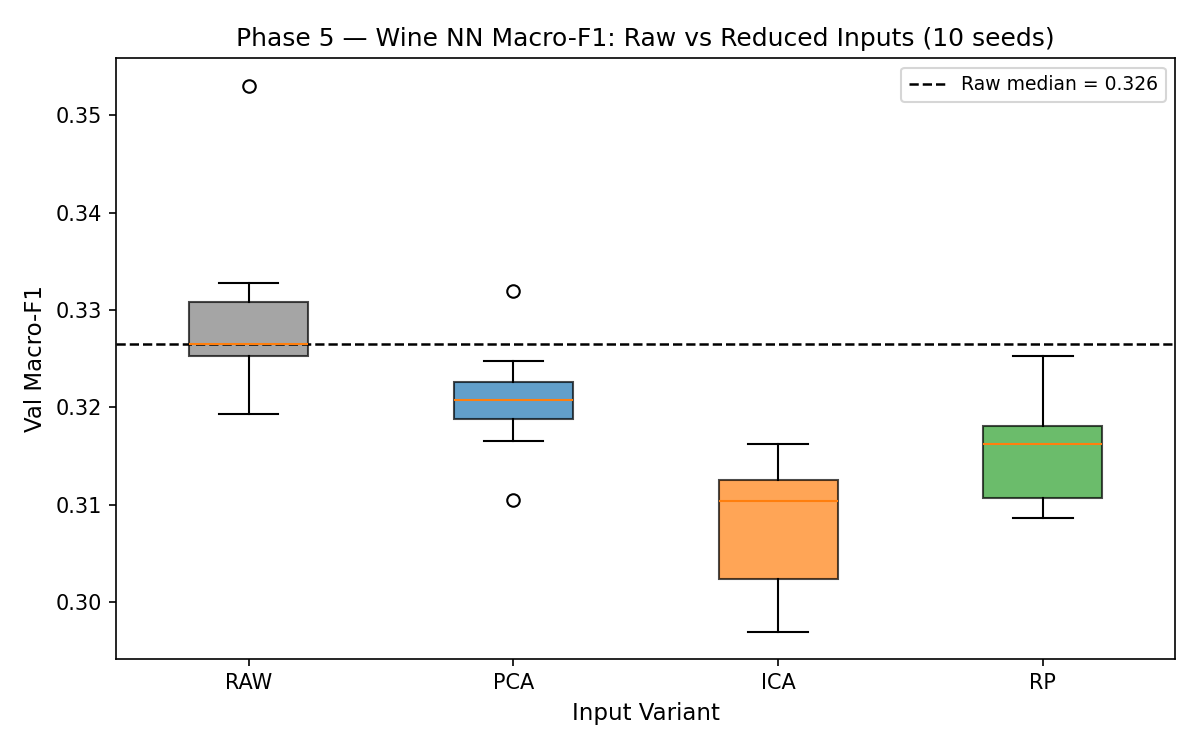
\includegraphics[width=\linewidth]{phase5_nn_reduced/phase5_f1_boxplot}
    \caption{Step 4: DR inputs}
  \end{subfigure}
  \hfill
  \begin{subfigure}{0.48\linewidth}
    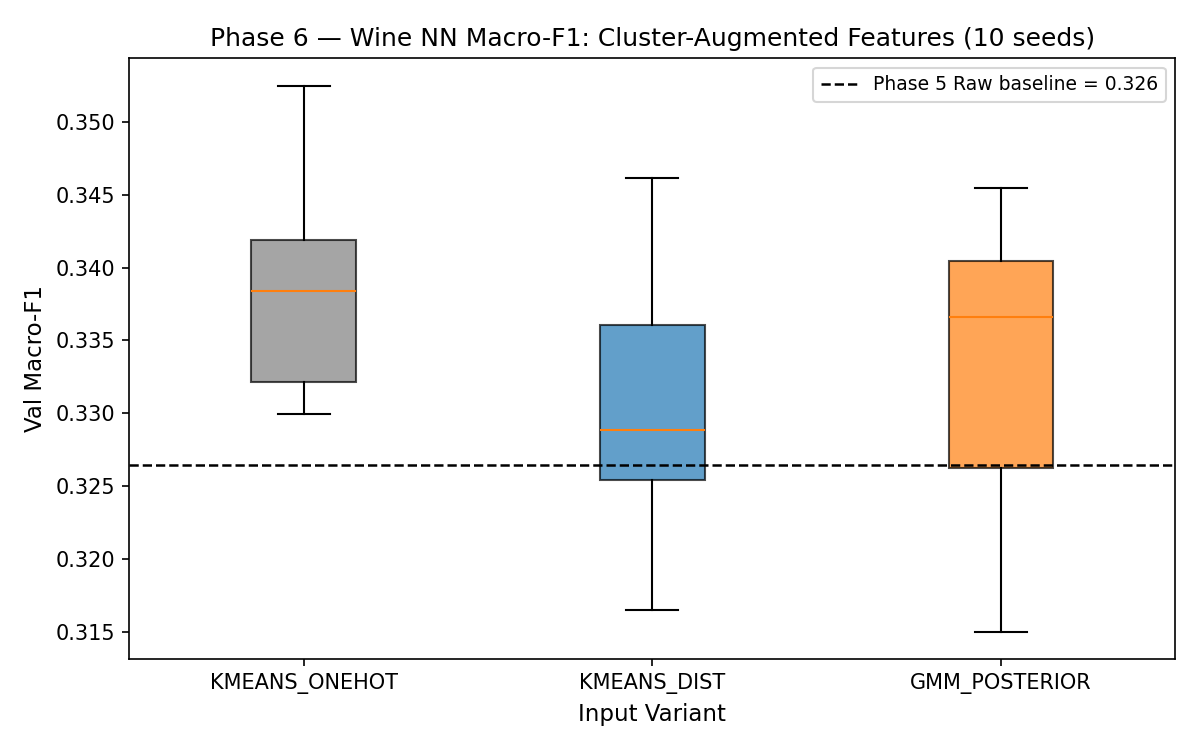
\includegraphics[width=\linewidth]{phase6_nn_cluster/phase6_f1_boxplot}
    \caption{Step 5: Cluster features}
  \end{subfigure}
  \caption{Macro-F1 distributions across 10 seeds.
  \textbf{Takeaway (left):} Every DR variant degrades performance relative to
  Raw; ICA's 4-d compression produces the lowest median, with the gap growing
  monotonically with compression severity.
  \textbf{Takeaway (right):} All three cluster augmentation variants exceed the
  Raw baseline; KMeans one-hot shows the highest and most stable gain.}
  \label{fig:f1_boxplots}
\end{figure}

\begin{figure*}[t]
  \centering
  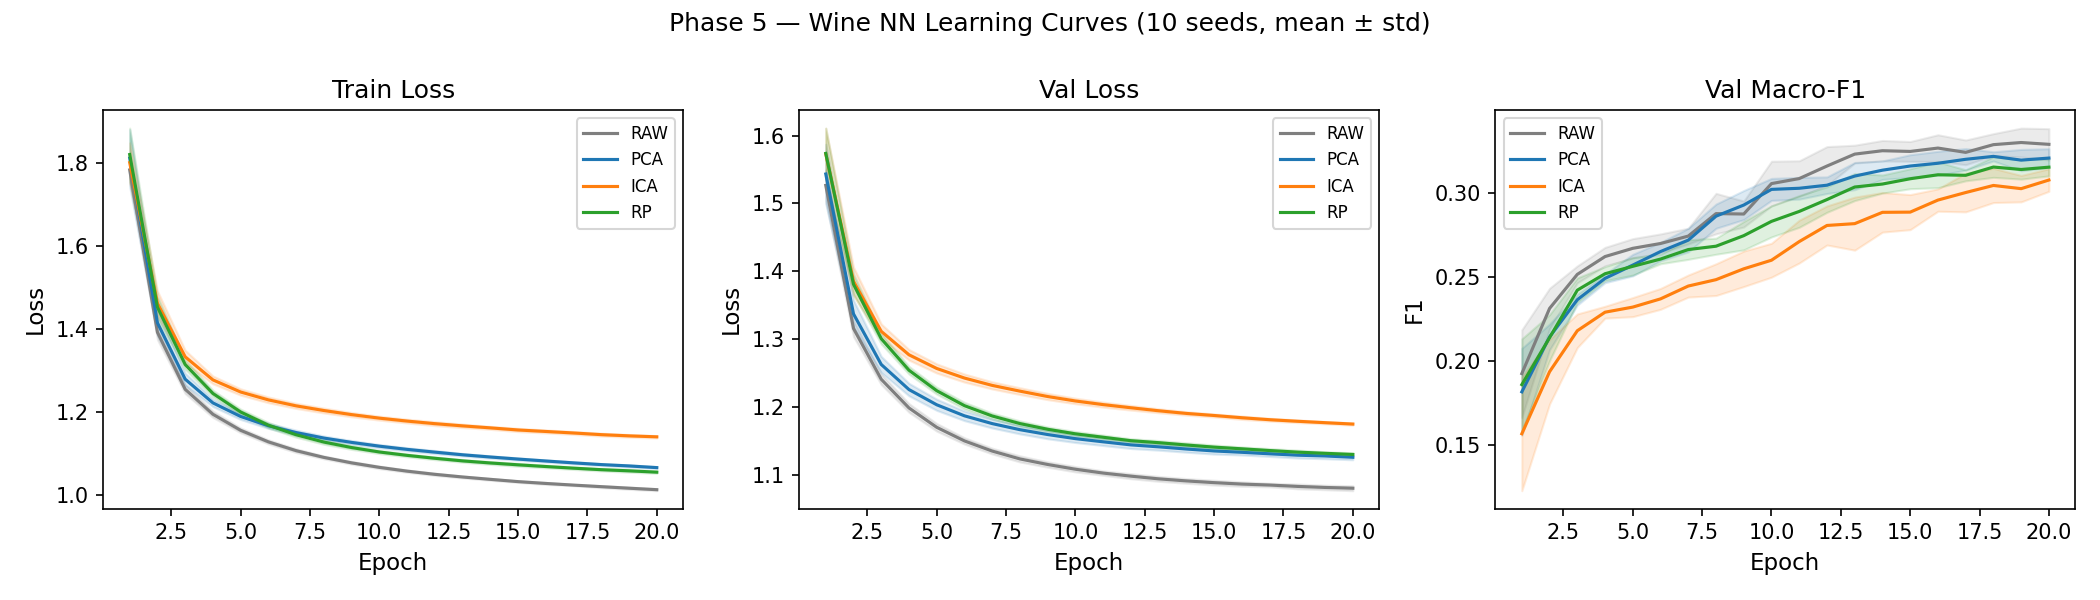
\includegraphics[width=0.92\textwidth]{phase5_nn_reduced/phase5_learning_curves}
  \caption{Learning curves across DR variants (mean $\pm$ 1\,SD, 10 seeds).
  \textbf{Takeaway:} All four variants converge to similar training-loss
  trajectories, confirming the architecture and optimizer are not bottlenecks.
  The validation F1 gap between Raw and ICA widens across all 20 epochs rather
  than closing, ruling out slower convergence as an explanation --- the ICA 4-d
  space genuinely lacks the capacity to encode adjacent quality classes.}
  \label{fig:learning_curves}
\end{figure*}

\subsection{Step 4 --- DR-Reduced Inputs}

Tables~\ref{tab:phase5} and Fig.~\ref{fig:f1_boxplots}(a) confirm the
information bottleneck prediction: every DR method degrades mean Macro-F1
relative to the 12-d raw baseline (0.329), and the degradation is strictly
ordered by compression severity.  PCA ($d\!=\!8$, $-2.5\%$) retains 93.7\% of
variance and causes the smallest loss.  RP ($d\!=\!8$, $-4.1\%$) operates at
the same dimensionality but without variance-optimized axes, discarding more
discriminative signal per dimension retained.  ICA ($d\!=\!4$, $-6.5\%$)
applies the most aggressive compression and produces the largest drop.

The learning curves in Fig.~\ref{fig:learning_curves} rule out slower
convergence as the cause: all variants reach similar training-loss values within
the first five epochs.  The validation F1 gap between Raw and ICA opens
immediately and widens steadily, indicating that the 4-d ICA space lacks the
representational capacity needed to separate adjacent quality grades, not merely
that it needs more epochs.  This result demonstrates that Wine's 12 features are
not redundant in the way Adult's OHE features are: each physicochemical
measurement carries distinct discriminative information, and removing any of them
has a measurable cost.

\textbf{Speed.}  Measured over 10 seeds at 20 epochs, reduced-input variants
complete in 0.26--0.27\,s mean (PCA/ICA/RP).  The raw 12-d baseline averages
0.42\,s, though this figure is inflated by PyTorch's one-time JIT compilation
cost incurred on the first forward pass of the run; after warmup the per-epoch
difference is $\sim$2--3\,ms.  Wine's training set (3{,}897 samples,
$\sim$30 batches per epoch) is small enough that per-dimension matrix
multiplication cost is swamped by Python interpreter and data-loading overhead.
A speed benefit from dimensionality reduction would be more pronounced on
larger datasets such as Adult, where the 104-to-22 compression reduces the
input layer computation by roughly $4.7\times$.

\subsection{Step 5 --- Cluster-Derived Feature Augmentation}

All three augmentation variants in Table~\ref{tab:phase6} exceed the raw
baseline, with the open-question resolving in favor of the hypothesis.  KMeans
one-hot (14d, mean F1\,=\,0.339, $+2.9\%$) provides the largest and most
stable gain.  The $K\!=\!2$ assignment encodes exactly the red/white partition
identified by KMeans in Step 1 and visualized in the t-SNE plots: it tells the
network which macro-cluster a sample belongs to, solving a structural
partitioning problem that would otherwise consume hidden-layer capacity.  With
that routing signal explicit, the network can devote its full representational
budget to resolving the fine-grained quality boundaries within each island.

GMM posterior (19d, $+1.3\%$) also improves performance but with higher seed
variance, because soft responsibilities from seven overlapping components blend
information from multiple regions of the feature space and do not provide a
crisp partition signal.  KMeans distances (14d, $+0.5\%$) produce the weakest
improvement: Euclidean distances to two centroids are highly collinear with the
original physicochemical features, adding little novel structural information
beyond what the raw 12 dimensions already encode.

The contrast between Steps~4 and~5 is the key finding of the NN experiments.
Removing features (DR) consistently hurts Wine's performance because the feature
set is already compact.  Adding cluster-derived features consistently helps
because they encode non-linear neighborhood structure that linear measurements do
not make explicit.

%%%%%%%%%%%%%%%%%%%%%%%%%%%%%%%%%%%%%%%%%%%%%%%%%%%%%%%%%%%%%%%%%%%%%%%%%%%%%%%%
\section{Extra Credit: t-SNE Visualization}

\begin{figure*}[t]
  \centering
  \begin{subfigure}{0.235\textwidth}
    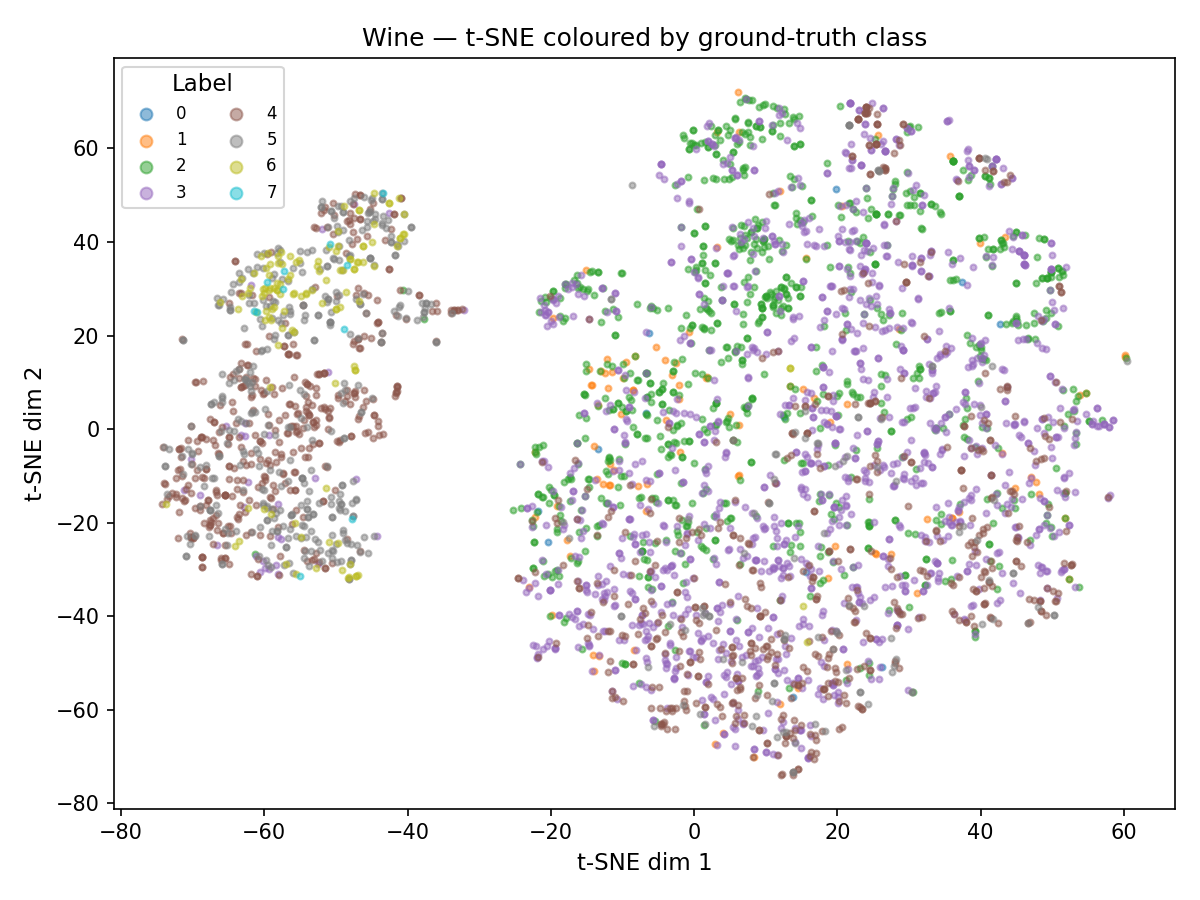
\includegraphics[width=\linewidth]{phase7_tsne/wine_tsne_labels}
    \caption{Wine, quality labels}
  \end{subfigure}
  \hfill
  \begin{subfigure}{0.235\textwidth}
    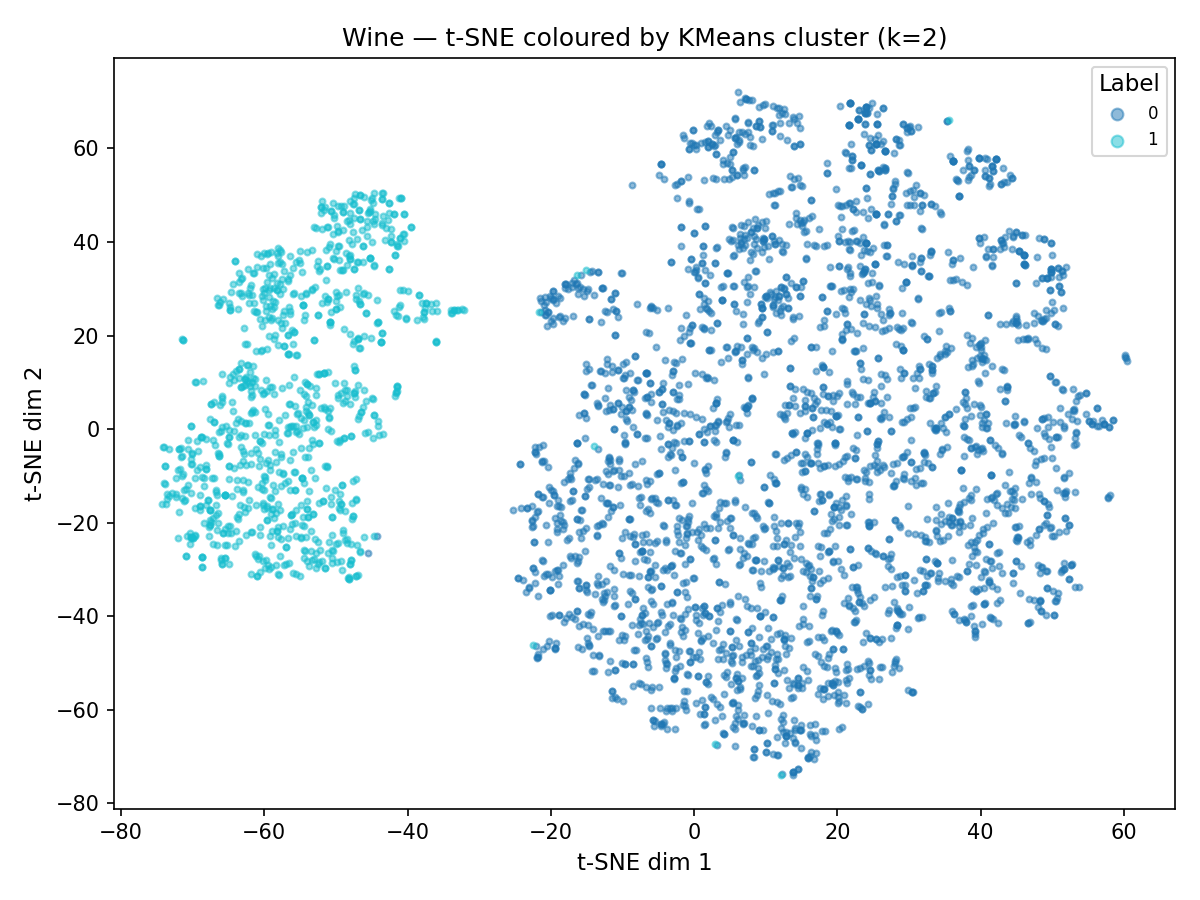
\includegraphics[width=\linewidth]{phase7_tsne/wine_tsne_clusters}
    \caption{Wine, KMeans ($K\!=\!2$)}
  \end{subfigure}
  \hfill
  \begin{subfigure}{0.235\textwidth}
    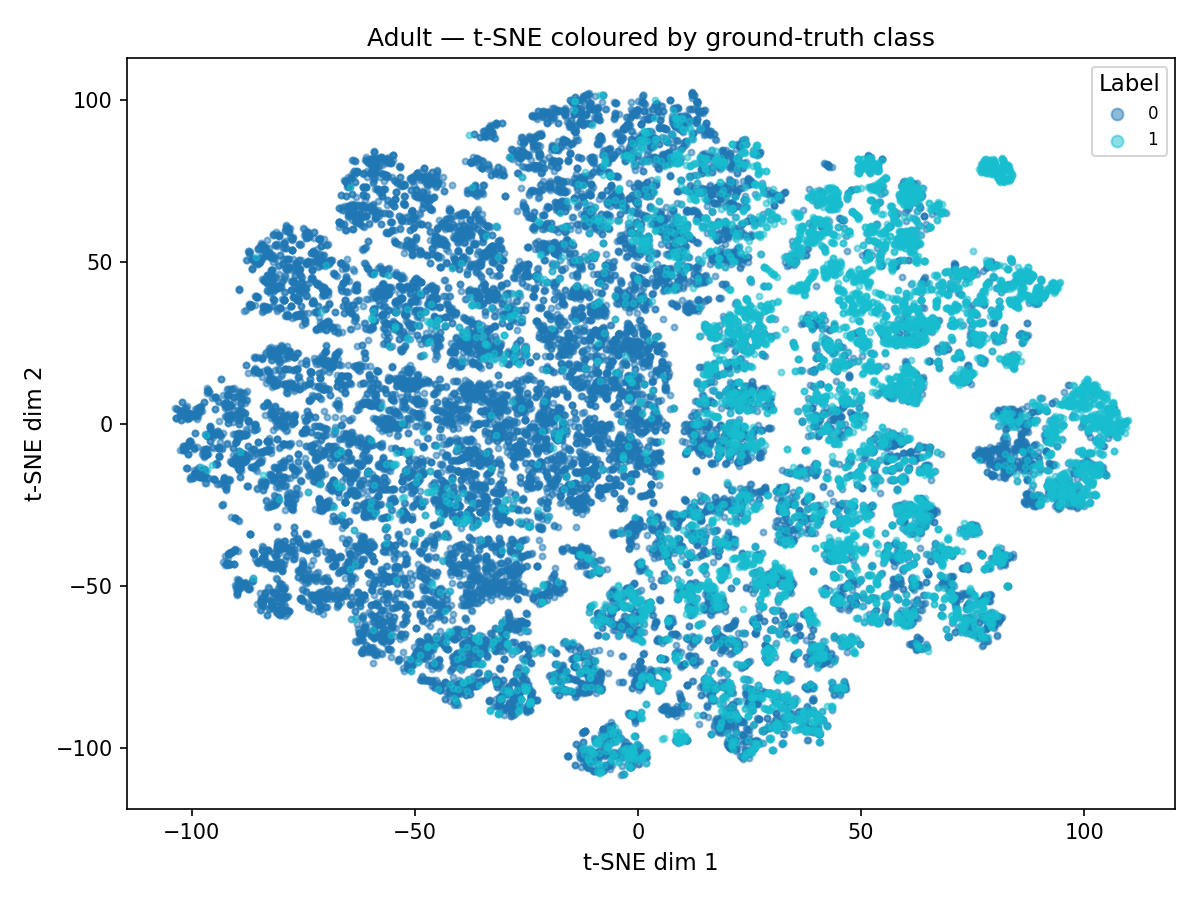
\includegraphics[width=\linewidth]{phase7_tsne/adult_tsne_labels}
    \caption{Adult, class labels}
  \end{subfigure}
  \hfill
  \begin{subfigure}{0.235\textwidth}
    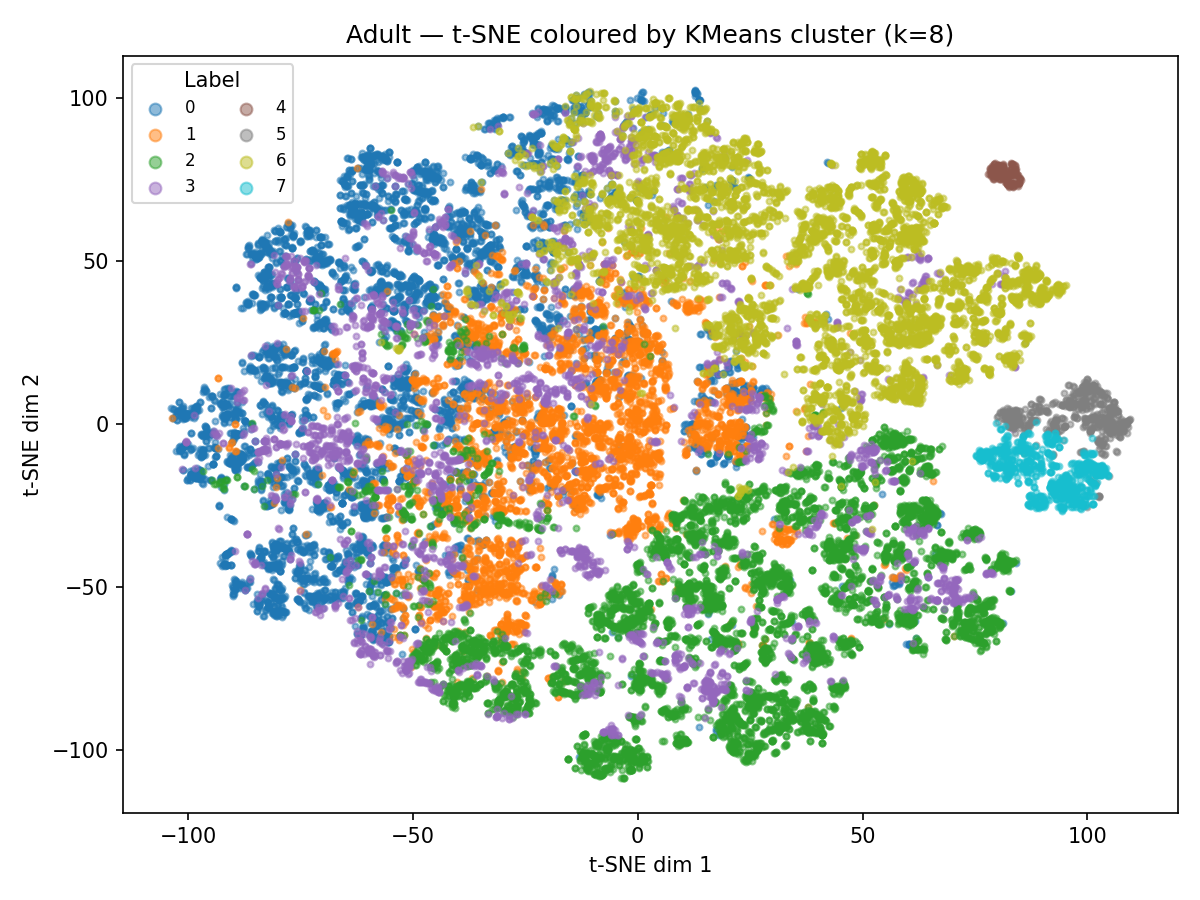
\includegraphics[width=\linewidth]{phase7_tsne/adult_tsne_clusters}
    \caption{Adult, KMeans ($K\!=\!8$)}
  \end{subfigure}
  \caption{t-SNE embeddings (perplexity\,=\,30, seed\,=\,42).
  Inter-cluster distances are not interpretable quantitatively.
  \textbf{Takeaway:} Wine (a, b) separates into two dense islands that
  KMeans $K\!=\!2$ identifies cleanly; quality labels are thoroughly mixed
  within each island --- visually confirming why DR hurts the NN (quality signal
  is diffuse across both clusters) and why KMeans one-hot helps (the
  macro-split is a clean, high-purity feature).  Adult (c, d) forms a single
  continuous manifold with no visible boundaries, explaining both the low raw
  silhouette and why PCA denoising is needed to expose latent cluster structure.}
  \label{fig:tsne}
\end{figure*}

t-SNE~\cite{vandermaaten2008} was applied to both training sets for qualitative
visualization only; embeddings are not used as feature inputs to any downstream
model.  The 2-D projections in Fig.~\ref{fig:tsne} corroborate every
quantitative finding in the report.  Wine's two-island structure (Figs.~a--b)
confirms that K-Means $K\!=\!2$ captures the dominant red/white partition.  The
complete mixing of quality colors within each island provides the strongest
visual evidence for the hypothesis: no projection --- linear or non-linear ---
can cleanly separate adjacent quality grades, because the class-label silhouette
of $-0.074$ means separation is geometrically impossible at any resolution.
Adult's continuous manifold (Figs.~c--d) illustrates the curse of dimensionality
in its 104-d OHE space: one-hot-encoded features form a connected surface that
does not fragment into discrete clusters, which is precisely why PCA compression
improves K-Means cluster quality by removing the sparse noise that inflates
Euclidean distances.

%%%%%%%%%%%%%%%%%%%%%%%%%%%%%%%%%%%%%%%%%%%%%%%%%%%%%%%%%%%%%%%%%%%%%%%%%%%%%%%%
\section{Conclusion}

The experiments confirm the hypothesis directionally across all five steps.
PCA improved Adult K-Means cluster quality by $23\%$ while Wine gained only
$4.7\%$, with the difference explained by Adult's $4.7\!\times$ compression
ratio versus Wine's $1.5\!\times$.  On Wine, every DR method degraded Macro-F1
in strict proportion to compression severity, confirming that Wine's 12 features
are compact and non-redundant.  Cluster-derived feature augmentation reversed
this trend: all three variants exceeded the raw baseline by encoding the latent
red/white partition that linear projections cannot make explicit.

The most unexpected result was Wine GMM under ICA ($+463\%$ silhouette), which
shows that the choice of DR method matters beyond compression efficiency.  ICA's
independence-maximizing projection amplifies non-Gaussian mixture structure that
PCA's variance-maximizing axes suppress.  When the downstream task is GMM
clustering, which also assumes a mixture model, the alignment between DR
objective and clusterer geometry provides a decisive advantage over generic
variance-based projection.

Two concrete algorithmic improvements would strengthen future iterations.  For
K-Means on Adult, replacing Euclidean distance with cosine similarity would
better respect the binary-sparse OHE geometry, where co-occurrence patterns are
more meaningful than $\ell_2$ norms inflated by the curse of dimensionality.
For Wine GMM, reducing the component count from 7 toward 2--3 would align the
generative model more closely with the macro-structure revealed by t-SNE,
likely improving hard-assignment silhouette at the cost of BIC log-likelihood.

\textbf{AI Use Statement.}  Once done with the preliminary draft, I used Claude Sonnet 4.6 to proofread and correct grammar, verify citation formatting, and make text concise where it was too verbose. I used GitHub Copilot to assist with figure alignment in LaTeX and to generate boilerplate code and bug fixes for the experiments and EDA code in the VS Code editor. I reviewed, verified, and understand all assisted content, and all analysis, interpretations, and conclusions are my own.

%%%%%%%%%%%%%%%%%%%%%%%%%%%%%%%%%%%%%%%%%%%%%%%%%%%%%%%%%%%%%%%%%%%%%%%%%%%%%%%%
\begin{thebibliography}{9}

\bibitem{kohavi1996}
R.~Kohavi, ``Scaling up the accuracy of naive-Bayes classifiers: A
decision-tree hybrid,'' in \emph{Proc. 2nd Int. Conf. Knowledge Discovery and
Data Mining (KDD)}, Portland, OR, 1996, pp.~202--207.

\bibitem{cortez2009}
P.~Cortez, A.~Cerdeira, F.~Almeida, T.~Matos, and J.~Reis, ``Modeling wine
preferences by data mining from physicochemical properties,'' \emph{Decision
Support Syst.}, vol.~47, no.~4, pp.~547--553, 2009.

\bibitem{hyvarinen2000}
A.~Hyv{\"a}rinen and E.~Oja, ``Independent component analysis: Algorithms and
applications,'' \emph{Neural Networks}, vol.~13, no.~4--5, pp.~411--430, 2000.

\bibitem{dempster1977}
A.~P.~Dempster, N.~M.~Laird, and D.~B.~Rubin, ``Maximum likelihood from
incomplete data via the EM algorithm,'' \emph{J. Royal Statistical Soc. Series
B}, vol.~39, no.~1, pp.~1--38, 1977.

\bibitem{jl1984}
W.~B.~Johnson and J.~Lindenstrauss, ``Extensions of Lipschitz mappings into a
Hilbert space,'' \emph{Contemporary Mathematics}, vol.~26, pp.~189--206, 1984.

\bibitem{lloyd1982}
S.~P.~Lloyd, ``Least squares quantization in PCM,'' \emph{IEEE Trans. Inf.
Theory}, vol.~28, no.~2, pp.~129--137, 1982.

\bibitem{vandermaaten2008}
L.~van der Maaten and G.~Hinton, ``Visualizing data using {t-SNE},''
\emph{J. Machine Learning Research}, vol.~9, pp.~2579--2605, 2008.

\end{thebibliography}

\end{document}
